\chapter{Návrh riešenia}

Pre použitie neurónových sietí v bežnej praxi doktorov pri diagnostike Alzheimerovej choroby je nevyhnutné, aby sa rozhodnutia neurónových sietí dali vysvetliť. Preto navrhujeme metódu na vyvsvetľovanie rozhodnutí neurónových sietí, ktorú overíme na MRI snímkoch u pacientov (CN, MCI a AD).

Vychádzajúc cieľa práce \textit{\ref{sec:goals_1} Vytvorenie novej, alebo vylepšenie existujúcej metódy pre vysvetľovanie rozhodnutí neurónových sietí} navrhujeme metódu, ktorá vychádza z už existujúcej metódy \textit{RISE} (Sek. \ref{sec:rise}). Táto metóda dosiahla veľmi dobré výsledky oproti metódam GradCAM a LIME a je teda vhodným základom na možné vylepšenia. Táto metóda funguje na pricípe zakrývania častí obrázka (tak ako iné perturbačné metódy). Po takomto prekrytí u iných perturbačných metódach vznikajú ostré hrany, čo môže neurónovú sieť mýliť, RISE tento problém ale nemá. Avšak tento prekryv býva zvyčajne v čiernej farbe. Keďže v MRI snímky sú v odtieňoch čiernej (a u AD jedincov je na snímkovch oveľa viac ''čiernej'' z dôvody úbytku mozgového tkaniva) môže byť práve toto ďaľším zdrojom zmätenia pre neurónovú sieť. Preto navrhujeme zakrývané miesta dokresliť určitou metódou spracovania obrazu (Sek. \ref{cap:image_processing}) alebo na zakrytie použiť inú hodnotu.

\section{RISEI - Randomized Input Sampling for Explanation with Inpainting}

Metódu sme pomenovali \textit{Randomized Input Sampling for Explanation with Inpainting} (tj. náhodné vzorkovanie vstupu pre vysvetlovanie s dokreslovaním) so skratkou \text{RISEI}.

Keďže metóda vychádza už z existujúcej metódy, časť našej metódy je samozrejme rovnaká. Proces vytvorenia vysvetlenia klasifikácie do triedy $T$ pre obrázok $O$ modelom je teda nasledovný:

\begin{enumerate}
    \item Vytvorenie \textit{N} náhodne zamaskovaných obrázkov z obrázka $O$
    \item Vloženie zamaskovaných obrázkov do modelu a následné získanie pravdepodobností pre triedu $T$
    \item Vytvorenie a vizualizácia vysvetlenia pomocou tepelnej mapy
\end{enumerate}

Toto sú 3 hlavné kroky z ktorých pozostáva táto metóda, ďalej bližšie popíšeme jednotlivé z nich.

\paragraph{Vytvorenie náhodne zamaskovaných obrázkov.}

Vytvorenie náhodne zamaskovaných obrázkov tiež pozostáva z niekoľkých krokov, pričom niektoré z nich môžu bežať paralelne. Tento sme znázornili diagramom (Obr. \ref{fig:risei_diagram}). Masky sa vytvárajú paralelne, pretože ''čierna'' maska ma jemné hrany a na dokreslenie potrebujeme naopak masku s ostrými hranami.

\begin{figure}[h!]
    \centering
    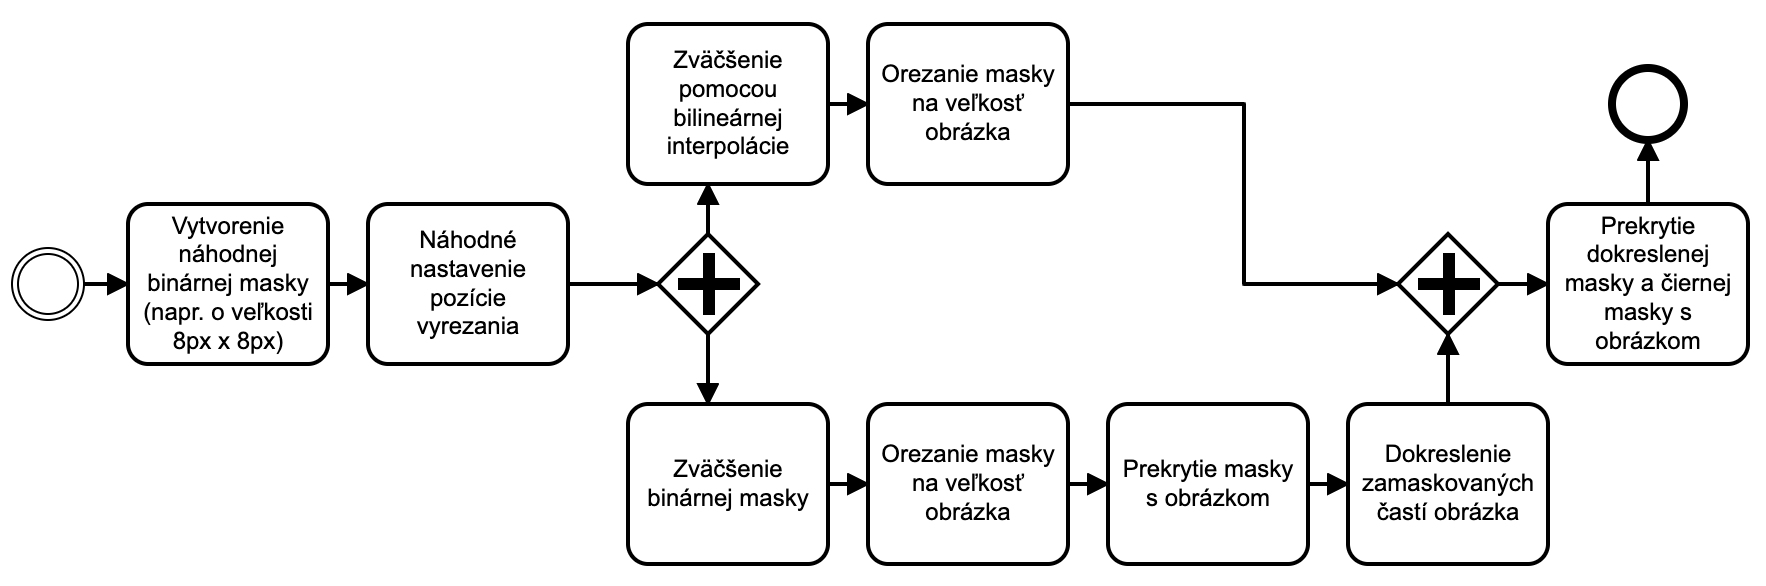
\includegraphics[scale=0.45]{assets/images/risei_diagram.png}
    \caption{BPMN diagram generovania jedného obrázka prekrytého maskou}
    \label{fig:risei_diagram}
\end{figure}

Oproti metóde \textit{RISE} vytvárame o jednu masku naviac a teda je originálny obrázok prekrytý z viacerými maskami. Jednotlivé masky cez seba prekryjeme, pričom každej z nich nastavíme určité množstvo priehľadnosti. S týmto pomerom môžeme ďalej experimentovať a výsledky porovnávať. Môžeme porovnať použitie iba dokreslenej masky s iba čiernou maskou a tiež s použitím oboch v rôznych pomeroch.

Vytvorenie ''čiernej'' masky je rovnaké ako pri metóde \textit{RISE}. Dokreslená maska vznikne dokreslením zakrytých (zamaskovaných) častí obrázka pomocou jedného z algoritmov na dokreslovanie (angl. inpainting). Tieto algoritmy sme popísali v sekcii \ref{cap:image_processing} Spracovanie obrazu. Obrázok \ref{fig:risei_inpainting_example} je príkladom dokreslenia častí vzorového obrázka na základe masky náhodne vygenerovanej masky. V našej metóde budeme experimentovať s rôznymi farbami prekrytia, nielen s čiernou.

\begin{figure}[h!]
    \centering
    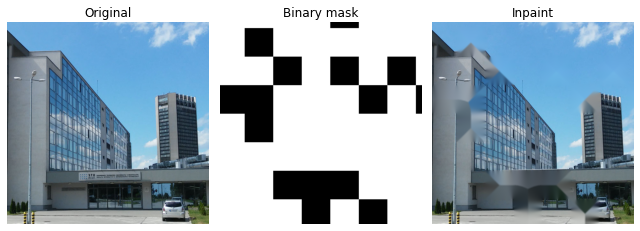
\includegraphics[width=13cm]{assets/images/risei_inpainting_example.png}
    \caption{Niektoré časti vzorového obrázoka (vľavo) boli dokreslené podľa náhodne vygenerovanej binárnej masky (v strede). Výsledný obrázok (vpravo) môže byť ešte prekrytý ''čiernou'' maskou s určitou priehľadnosťou.}
    \label{fig:risei_inpainting_example}
\end{figure}

\paragraph{Vytvorenie a vizualizácia vysvetlenia pomocou tepelnej mapy.}

Tento krok je identický s originálnou metódou \textit{RISE}. Nasledovný vzorec \ref{eq:risei_heatmap_1} vyjadruje výpočet dôležitosti $I$ pre každý pixel $[x, y]$ obrázka, kde $n$ je počet všetkých zamaskovaných obrázkov. Funkcia $p(k, x, y)$ vracia $0$ ak pixel $[x, y]$ bol v danom zamaskovanom obrázku $k$ prekrytý, inak vracia predikciu (pravdepodobnosť) z modelu pre zamaskovaný obrázok $k$.

\begin{equation}
    I_{x, y} = \frac{\sum_{k}^{n} p(k, x, y)}{n}
    \label{eq:risei_heatmap_1}
\end{equation}

Táto metóda do orignálnej pridáva niekoľko parametrov, a najmä výpočtovo náročné dokreslovanie, preto bude nutné nájsť vhodné nastavenie parametrov aby výpočet vysvetlenia nebol príliš časovo náročný. Práve výpočtová náročnosť môže byť slabinou tejto metódy.

\section{Overenie riešenia}

Našu metódu budeme najskôr porovnávať s originálnou metódou RISE (tj. či sa nám podarilo spraviť lepšiu metódu) a následne s metódou LRP. Tieto experimenty môžeme vykonávať na CN a AD vzorkách; a aj na CN, MCI a AD vzorkách. Budeme sledovať kvalitu navrhnutej metódy (oproti ostatným metódam) a na základe týchto tepelných máp budeme vyhodnocovať mieru správnosti modelu.

\subsection{Dátová sada} Experimenty budeme vykonávať na dátovej sade ADNI, ktorá obsauje MRI snímky AD pacientov. Táto dátova sada bola použitá aj na trénovanie state-of-the-art modelu na diagnsotiku Alzheimerovej choroby \cite{esmaeilzadeh2018end}, ale aj pri vysvetlovaní rozhodnutí neurónovej siete pomocou LRP \cite{bohle2019layer}. Na tejto dátovej sade budeme musieť vykonáť rovnaké predspracovanie ako \citeauthor*{bohle2019layer} aby sme sa s ich výsledkami mohli porovnať. Prípadne môžeme vykonať vlastné predspracovanie, ale budeme musieť vykonať aj experimenty s metódou LRP.

\subsection{Experimenty}

Najskôr budeme vyhodnocovať nami navrhnutú metódu pomocou sledovania kvality tepelných máp. Následne budeme overovať správnosť modelu pomocou nami navrhnutej metódy.

\subsubsection{Určenie kvality metódy vysvetľovania rozhodnutí modelu}

Kvalitu metódy vysvetľovania rozhodnutí modelu budeme sledovať určovaním kvality tepelnej mapy. Tá v kontexte našej práce hovorí o tom, do akej miery táto mapa odzrkadluje to, na základe čoho sa model rozhoduje. Toto budeme merať metrikami \textit{insertion (AUC)} a \textit{deletion (AUC)}, ktoré sme bližšie popísali v sekcii \ref{sec:rise}. Táto metrika nám povie ako dobrá je naša metóda na vysvetlovanie.

\subsubsection{Určenie správnosti modelu}

Správnosť modelu budeme určovať na na základe tepelných máp vytvorených pomocou metódy na vysvetľovanie predikcií modelu. Budeme overovať do akej miery dávajú tepelné mapy zmysel v kontexte skutočnej anatómie mozgu. Sledujeme, že či tepelná mapa nehovorí o tom, že sa model rozhodol na základe takej oblasti mozgu, z ktorej sa Alzheimerova choroba nedá zistiť. Veľkú úlohu v tejto metrike teda zohráva aj kvalita natrénovaného modelu. Táto metrika je súborom niekoľkých metrík z práce od \citeauthor*{bohle2019layer}.

% TODO: tell more about those metrics, ffs

\section{Záver}

V tejto kapitole sme navrhli metódu na vysvetľovanie rozhodnutí modelov strojového učenia a spôsob jej implementácie. Navrhnutú metódu budeme overovať na neurónových sieťach detekujúcich Alzheimerovu chorobu s cieľom odhalovania nesprávnych rozhodnutí.
